\chapter{\textit{Positive-Unlabeled Learning}}\label{chap:pu_learning}

% Este capítulo estudia la aplicación de \textit{PU learning} a la predicción de hemorragia y neumotórax. Las formulaciones evaluadas se comparan con el aprendizaje supervisado sobre representaciones tabulares y volúmenes tridimensionales, analizando tanto su rendimiento como sus principales limitaciones.

% \section{Objetivo y planteamiento del análisis}

% Las etiquetas positivas corresponden a pacientes cuya complicación fue detectada, diagnosticada y registrada durante la atención hospitalaria y, cuando fue necesario, tratada. Sin embargo, la ausencia de una complicación registrada no garantiza necesariamente que esta no se produjera. Algunas hemorragias de pequeña magnitud o neumotórax leves podrían haber pasado inadvertidos o no haber quedado recogidos en el registro clínico. Por este motivo, los pacientes sin una complicación documentada pueden considerarse casos no etiquetados, en lugar de negativos confirmados, en las formulaciones de \textit{PU learning}. Si este conjunto contiene positivos no identificados, su tratamiento sistemático como negativos puede desplazar la frontera de decisión y dificultar el reconocimiento de pacientes con características similares.

% A partir de esta motivación, el análisis ha evaluado si el tratamiento mediante \textit{PU learning} de los pacientes sin una complicación registrada modifica el rendimiento respecto al aprendizaje supervisado convencional. La hemorragia y el neumotórax se han estudiado como objetivos binarios independientes sobre representaciones clínicas y geométricas, radiómicas, combinadas y volumétricas. La hipótesis ha sido que el tratamiento específico del conjunto no etiquetado podría favorecer la detección de posibles positivos no identificados, aunque a costa de una menor especificidad o una peor calibración. En la extensión tridimensional se ha incorporado nnPU como formulación de riesgo no negativo.

Este capítulo evalúa si considerar como no etiquetados, en lugar de como negativos, a los pacientes sin una complicación registrada mejora la predicción de hemorragia y neumotórax, dado que algunos casos leves podrían haber pasado inadvertidos o no haberse documentado. Ambos objetivos se analizan por separado sobre representaciones clínicas y geométricas, radiómicas, combinadas y volumétricas. Para ello, se comparan formulaciones de PU learning con el aprendizaje supervisado, bajo la hipótesis de que podrían recuperar positivos no identificados, aunque con una posible pérdida de especificidad o calibración. En el análisis tridimensional se incorpora además nnPU, una formulación basada en riesgo no negativo.

\section{Datos y representaciones de entrada}

El análisis tabular se ha realizado sobre la cohorte PU definida en la Tabla~\ref{tab:resumen_cohortes}. Las tres representaciones comparadas han utilizado los mismos pacientes y las mismas particiones, de modo que sus diferencias no están condicionadas por cambios en la composición de la muestra. En esta cohorte se han registrado 48 casos de hemorragia y 63 de neumotórax. Para cada objetivo, los pacientes con la complicación confirmada se han considerado positivos y los restantes han formado el conjunto no etiquetado.

Se han definido tres representaciones de entrada. La primera ha reunido 32 variables clínicas y geométricas, incluyendo la edad, los antecedentes clínicos preprocedimentales y las medidas de tamaño y profundidad pleural del nódulo definidas en el Capítulo~\ref{chap:subgroup_discovery}. La segunda ha contenido 321 características radiómicas de primer orden, forma y textura extraídas de las máscaras de pulmón, nódulo y vasos según el procedimiento presentado en el Capítulo~\ref{chap:radiomica}. La tercera ha combinado ambos bloques en una representación de 353 variables. De este modo, se ha podido estudiar si el comportamiento de las formulaciones PU depende del tipo de información disponible y si la integración de datos clínicos, geométricos y radiómicos aporta alguna ventaja.

Como extensión del análisis tabular, también se ha estudiado el aprendizaje PU directamente sobre imagen tridimensional. Esta rama ha utilizado la cohorte tridimensional definida en la Tabla~\ref{tab:resumen_cohortes}, en la que 47 pacientes presentaban hemorragia y 63 neumotórax. Su diferencia respecto a la cohorte tabular se debe a la disponibilidad de las entradas volumétricas.

% El identificador del paciente se ha utilizado únicamente para alinear las tablas y no se ha incluido como predictor. También se han excluido los metadatos técnicos de las imágenes y la variable \texttt{Sexo\_binaria}, siguiendo el criterio clínico adoptado en los análisis anteriores, mientras que la variable \texttt{Edad} se ha conservado. Las operaciones de imputación, escalado y transformación necesarias para cada modelo se han ajustado posteriormente dentro de las particiones de entrenamiento, como se detalla en la sección metodológica.

\section{Metodología}

La comparación incluye dos referencias supervisadas y dos métodos que tratan explícitamente el conjunto no etiquetado. La diferencia operativa entre las cuatro formulaciones se resume en la Sección~\ref{sec:pu_formulaciones}.

\subsection{Formulaciones evaluadas}\label{sec:pu_formulaciones}

A continuación se describen las cuatro formulaciones evaluadas:
% El aprendizaje supervisado convencional se ha utilizado como referencia, considerando negativos a todos los pacientes sin la complicación analizada. También se ha incluido una formulación PU ingenua que, aunque denomina a estos pacientes no etiquetados, los trata provisionalmente como negativos durante el entrenamiento. Por tanto, ambas formulaciones son equivalentes cuando utilizan los mismos datos, modelos y semillas. Esta comparación se ha mantenido como control para comprobar que las diferencias observadas en los demás métodos PU proceden de sus mecanismos específicos y no de cambios accidentales en la implementación.

% Como segunda referencia, se ha evaluado un modelo supervisado con negativos fiables. En esta formulación, el entrenamiento se ha restringido a los positivos observados y a los pacientes con la etiqueta \texttt{Sin\_complicación}, que se han considerado negativos con mayor certeza. Los pacientes que presentaban otras complicaciones, pero no la complicación objetivo, se han excluido del ajuste para evitar asumir directamente que constituyen negativos fiables.

% Las dos formulaciones PU específicas han sido la corrección de Elkan-Noto y Bagging PU. La primera ha entrenado el clasificador distinguiendo positivos observados y no etiquetados y ha corregido posteriormente sus puntuaciones mediante una estimación interna de \(c\). En Bagging PU se han ajustado 15 clasificadores. Cada uno ha utilizado todos los positivos observados y una muestra aleatoria del conjunto no etiquetado del mismo tamaño que el grupo positivo. La puntuación final se ha obtenido promediando las salidas de los 15 modelos, reduciendo así la dependencia de una única selección de ejemplos no etiquetados.

\begin{itemize}
    \item \textbf{Supervisado convencional:} todos los pacientes sin la complicación analizada se han considerado negativos.

    % \item \textbf{Supervisado con negativos fiables:} el entrenamiento se ha restringido a los positivos observados y a los pacientes con la etiqueta \texttt{Sin\_complicación}, utilizados como negativos.

    \item \textbf{Supervisado con etiquetado negativo ingenuo:} el entrenamiento se ha restringido a los positivos observados y a los pacientes pertenecientes al estado derivado sin complicaciones, correspondiente a \((0,0)\), que se han considerado negativos bajo una suposición simplificadora.

    % \item \textbf{PU ingenuo:} los casos no etiquetados se han tratado provisionalmente como negativos. Por tanto, esta formulación es equivalente al aprendizaje supervisado convencional cuando se mantienen los mismos datos, modelos y semillas, y se ha incluido como control de implementación.

    \item \textbf{Elkan-Noto:} las puntuaciones obtenidas al distinguir positivos observados y casos no etiquetados se han corregido mediante una estimación interna de la probabilidad de etiquetado \(c\), definida en la Sección~\ref{sec:fundamentos_pu}.

    \item \textbf{Bagging PU:} se han ajustado 15 clasificadores utilizando todos los positivos observados y distintas muestras del conjunto no etiquetado. La puntuación final se ha calculado promediando sus salidas.
\end{itemize}


\subsection{Modelos y preprocesamiento}

Se han considerado nueve familias de clasificadores: regresión logística, SVM lineal y con núcleo RBF, Random Forest, Extra Trees, LightGBM, XGBoost, HistGradientBoosting y perceptrón multicapa. Esta variedad ha permitido comparar modelos lineales y no lineales, \textit{ensembles} y una red neuronal tabular sin fijar de antemano una única familia para todas las modalidades y objetivos.

Cada clasificador se ha integrado en un \textit{pipeline} compuesto por imputación mediante la mediana, eliminación de variables con varianza nula y estandarización. En cada partición, este flujo se ha ajustado con los datos de entrenamiento y se ha aplicado sin reajuste a los datos de validación o prueba correspondientes. Cuando el clasificador proporcionaba probabilidades se ha utilizado la salida de la clase positiva, mientras que en los modelos basados en una función de decisión, esta se ha transformado al intervalo \([0,1]\) mediante una función logística.

\subsection{Estimación de la probabilidad de etiquetado}
En cada iteración externa, \(\hat{c}\), correspondiente al parámetro \(c\) definido en la Sección~\ref{sec:fundamentos_pu}, se ha estimado a partir de predicciones internas del conjunto de entrenamiento externo. Para generarlas, este conjunto se ha dividido en cuatro \textit{folds} internos y cada uno se ha evaluado mediante un modelo ajustado con los tres restantes. A continuación, \(\hat{c}\) se ha calculado como la puntuación media asignada a los positivos observados:

\[
\hat{c}
=
\frac{1}{|P|}
\sum_{i\in P} g_{\mathrm{OOF}}(\mathbf{x}_i),
\]

donde \(P\) es el conjunto de positivos observados del entrenamiento externo y \(g_{\mathrm{OOF}}(\mathbf{x}_i)\) es la puntuación interna asignada al paciente \(i\). Las puntuaciones obtenidas posteriormente en el test externo se han corregido dividiéndolas por \(\hat{c}\) y limitando el resultado al intervalo \([0,1]\), de acuerdo con la expresión presentada en la Sección~\ref{sec:fundamentos_pu}.

\subsection{Selección del umbral de decisión}

El umbral no se ha fijado en 0,5, sino que se ha seleccionado a partir de las predicciones de la validación interna. Para cada configuración se han evaluado sus puntuaciones observadas hasta un máximo de 201 puntos y se ha elegido el umbral con mayor G-mean de sensibilidad y especificidad. Los empates se han resuelto, por este orden, mediante el coeficiente de correlación de Matthews (MCC) y F1. El umbral seleccionado se ha aplicado sin cambios al test externo.

\section{Diseño experimental}

El experimento se ha organizado como un diseño factorial de dos complicaciones, tres representaciones de entrada y cuatro formulaciones, dando lugar a 24 combinaciones experimentales. En todas ellas se han mantenido la misma cohorte, las mismas particiones externas y la misma semilla, lo que ha permitido realizar comparaciones emparejadas entre métodos.

\subsection{Validación anidada}\label{subsec:validacion_pu_tabular}

Los experimentos tabulares se han evaluado mediante la validación cruzada anidada representada en la Figura~\ref{fig:validacion_pu_tabular}. Los 205 pacientes se han distribuido en cinco \textit{folds} externos estratificados según las combinaciones de etiquetas. En cada iteración, un \textit{fold} de 41 pacientes se ha reservado como test externo y los cuatro restantes, formados por 164 pacientes, han constituido el entrenamiento externo.

\begin{figure}[!htbp]
    \centering
    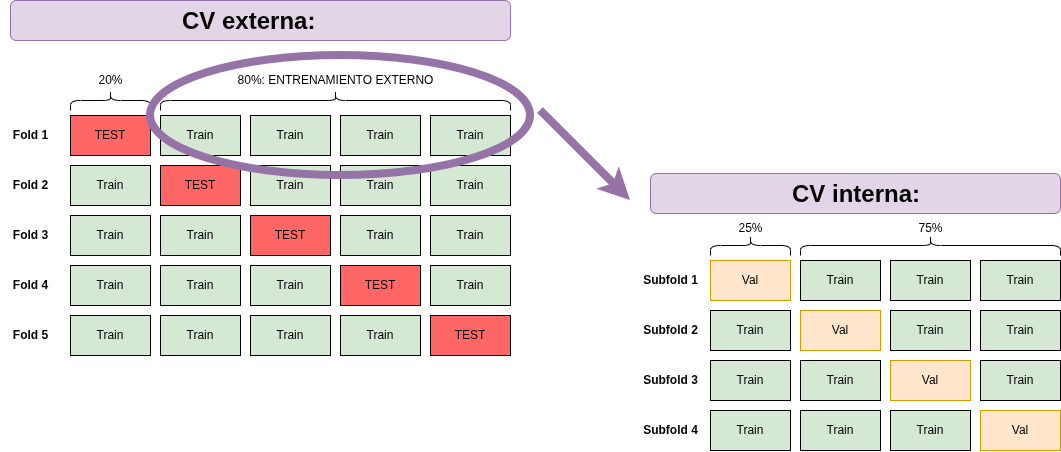
\includegraphics[width=\textwidth]{imagenes/pu_learning/CV_anidada.png}
    \caption{Esquema de validación anidada empleado en los experimentos tabulares de \textit{PU learning}.}
    \label{fig:validacion_pu_tabular}
\end{figure}

% Dentro de cada entrenamiento externo se ha realizado una validación cruzada interna de cuatro \textit{folds}. Para cada una de las 64 configuraciones candidatas, la validación cruzada interna ha generado una predicción para cada paciente del entrenamiento externo. Cada predicción ha sido realizada por un modelo entrenado con los otros tres \textit{folds} internos, por lo que el paciente evaluado no ha participado en el ajuste de ese modelo. A partir del conjunto de estas predicciones se ha calculado el \textit{average precision} de cada configuración y se ha seleccionado aquella con el valor más alto. En caso de empate se han utilizado, sucesivamente, G-mean, MCC y el índice de la configuración como criterios de desempate. Estas mismas predicciones internas se han utilizado para estimar c y seleccionar el umbral de decisión mediante los procedimientos descritos anteriormente.

Dentro de cada entrenamiento externo se ha realizado una validación cruzada interna de cuatro \textit{folds}. Las predicciones internas agregadas se han utilizado para evaluar las 64 configuraciones candidatas y seleccionar una de ellas conforme a los criterios descritos en la Subsección~\ref{subsec:metricas_pu}. Estas mismas predicciones también se han utilizado para estimar \(c\) y seleccionar el umbral de decisión mediante los procedimientos descritos anteriormente.


Una vez seleccionada la configuración, el modelo se ha ajustado con los 164 pacientes del entrenamiento externo y se ha evaluado una única vez sobre los 41 pacientes del test externo. Este proceso se ha repetido para los cinco \textit{folds}, de manera que cada paciente ha formado parte del test externo exactamente una vez. Finalmente, las predicciones externas se han unido para calcular las métricas OOF sobre los 205 pacientes.

\subsection{Espacio de configuraciones}

El espacio de búsqueda ha incluido 64 configuraciones: 8 de regresión logística, 8 de SVM lineal, 6 de SVM con núcleo RBF, 12 de Random Forest, 12 de Extra Trees, 4 de LightGBM, 4 de XGBoost, 4 de HistGradientBoosting y 6 de perceptrón multicapa. Dentro de cada familia se han variado los principales hiperparámetros de regularización, complejidad, ponderación de clases y tamaño del modelo. Este mismo espacio se ha evaluado en cada combinación de complicación, representación y formulación, sin seleccionar configuraciones a partir de los \textit{folds} externos.

% En conjunto, el diseño ha comprendido:
% \[
% 2\ \text{complicaciones}
% \times 3\ \text{representaciones}
% \times 4\ \text{formulaciones}
% =24\ \text{combinaciones experimentales},
% \]

% cada una con cinco evaluaciones externas y una comparación interna de las 64 configuraciones.

\subsection{Métricas de evaluación}
\label{subsec:metricas_pu}

La métrica principal para la selección interna de las configuraciones ha sido el \textit{average precision}, que resume la relación entre precisión y sensibilidad para los distintos umbrales de decisión. Esta métrica resulta especialmente adecuada ante el desequilibrio entre positivos y no etiquetados, ya que permite evaluar la capacidad del modelo para asignar puntuaciones superiores a los positivos observados.

En cada entrenamiento externo, se ha calculado el \textit{average precision} de las 64 configuraciones candidatas a partir de sus predicciones internas agregadas y se ha seleccionado la configuración con el valor más alto. En caso de empate se han empleado, sucesivamente, G-mean, el MCC y el índice de la configuración. Como medida complementaria independiente del umbral se ha calculado el área bajo la curva ROC.

Tras aplicar el umbral seleccionado internamente, se han calculado F1, precisión, sensibilidad, especificidad, valor predictivo negativo, \textit{balanced accuracy}, G-mean y MCC. También se han conservado los recuentos de verdaderos positivos, falsos positivos, verdaderos negativos y falsos negativos, así como el número de positivos predichos. Finalmente, el Brier score se ha utilizado para evaluar el error de las probabilidades, donde un valor menor indica una mayor proximidad entre las puntuaciones predichas y las etiquetas observadas. La interpretación se ha realizado considerando conjuntamente discriminación, equilibrio entre clases y calibración, evitando concluir a partir de una única métrica.

\section{Resultados}

En esta sección se presentan y comparan los resultados obtenidos por las distintas configuraciones evaluadas.

\subsection{Comparación global de las formulaciones}

No se ha observado una formulación PU que supere de forma consistente al aprendizaje supervisado en ambos objetivos y en las tres representaciones. Bagging PU ha proporcionado algunas mejoras moderadas en discriminación o equilibrio entre clases, mientras que Elkan-Noto ha resultado competitivo principalmente con las variables clínicas y geométricas. En cambio, la corrección de Elkan-Noto ha incrementado de forma marcada el Brier score en todas las modalidades, indicando un mayor error de las probabilidades corregidas respecto a las etiquetas observadas. El etiquetado negativo ingenuo también ha mostrado un comportamiento dependiente de la complicación: ha reducido generalmente el rendimiento en hemorragia, pero ha sido competitivo en neumotórax.

\subsection{Resultados por complicación}

En hemorragia (Tabla~\ref{tab:pu_resultados_hemorragia}), Bagging PU con la representación combinada obtuvo el mayor \textit{average precision} (0,445 frente a 0,428 del supervisado equivalente), pero no mejoró G-mean ni MCC. Elkan–Noto con variables clínicas y geométricas lideró AUC-ROC, F1, G-mean y MCC (0,673; 0,478; 0,653; 0,292), a costa de reducir el average precision a 0,370 y elevar el Brier score a 0,493. Por tanto, ninguna mejora dependiente del umbral se tradujo a la vez en mejor ordenación y mejor calidad probabilística.

\begin{table}[!htbp]
\centering
\caption{Resultados OOF para hemorragia. AP: \textit{average precision}; AUC: área bajo la curva ROC; Sens.: sensibilidad; Esp.: especificidad.}
\label{tab:pu_resultados_hemorragia}
\scriptsize
\begin{adjustbox}{max width=\textwidth}
\begin{tabular}{llcccccccc}
\toprule
\textbf{Representación} & \textbf{Formulación} & \textbf{AP} & \textbf{AUC} & \textbf{F1} & \textbf{Sens.} & \textbf{Esp.} & \textbf{G-mean} & \textbf{MCC} & \textbf{Brier} \\
\midrule
Clínica+geom. & Supervisado & 0,422 & 0,646 & 0,431 & 0,458 & 0,796 & 0,604 & 0,245 & 0,197 \\
Clínica+geom. & Etiq. neg. ingenuo & 0,352 & 0,630 & 0,403 & 0,521 & 0,675 & 0,593 & 0,172 & 0,223 \\
Clínica+geom. & Elkan-Noto & 0,370 & 0,673 & 0,478 & 0,562 & 0,758 & 0,653 & 0,292 & 0,493 \\
Clínica+geom. & Bagging PU & 0,372 & 0,663 & 0,457 & 0,604 & 0,682 & 0,642 & 0,249 & 0,236 \\
\midrule
Radiómica & Supervisado & 0,416 & 0,654 & 0,426 & 0,542 & 0,694 & 0,613 & 0,208 & 0,174 \\
Radiómica & Etiq. neg. ingenuo & 0,370 & 0,623 & 0,404 & 0,438 & 0,777 & 0,583 & 0,204 & 0,200 \\
Radiómica & Elkan-Noto & 0,309 & 0,588 & 0,423 & 0,604 & 0,618 & 0,611 & 0,190 & 0,365 \\
Radiómica & Bagging PU & 0,396 & 0,645 & 0,452 & 0,583 & 0,694 & 0,636 & 0,243 & 0,238 \\
\midrule
Combinada & Supervisado & 0,428 & 0,657 & 0,462 & 0,625 & 0,669 & 0,647 & 0,254 & 0,174 \\
Combinada & Etiq. neg. ingenuo & 0,379 & 0,637 & 0,439 & 0,521 & 0,739 & 0,620 & 0,235 & 0,204 \\
Combinada & Elkan-Noto & 0,294 & 0,593 & 0,408 & 0,604 & 0,586 & 0,595 & 0,162 & 0,467 \\
Combinada & Bagging PU & 0,445 & 0,671 & 0,450 & 0,604 & 0,669 & 0,636 & 0,236 & 0,237 \\
\bottomrule
\end{tabular}
\end{adjustbox}
\end{table}

En neumotórax, cuyos resultados se muestran en la Tabla~\ref{tab:pu_resultados_neumotorax}, el mayor \textit{average precision} ha correspondido al modelo con etiquetado negativo ingenuo y representación combinada, con 0,410.

\begin{table}[!htbp]
\centering
\caption{Resultados OOF para neumotórax. AP: \textit{average precision}; AUC: área bajo la curva ROC; Sens.: sensibilidad; Esp.: especificidad.}
\label{tab:pu_resultados_neumotorax}
\scriptsize
\begin{adjustbox}{max width=\textwidth}
\begin{tabular}{llcccccccc}
\toprule
\textbf{Representación} & \textbf{Formulación} & \textbf{AP} & \textbf{AUC} & \textbf{F1} & \textbf{Sens.} & \textbf{Esp.} & \textbf{G-mean} & \textbf{MCC} & \textbf{Brier} \\
\midrule
Clínica+geom. & Supervisado & 0,340 & 0,532 & 0,412 & 0,524 & 0,549 & 0,536 & 0,068 & 0,240 \\
Clínica+geom. & Etiq. neg. ingenuo & 0,387 & 0,593 & 0,524 & 0,794 & 0,451 & 0,598 & 0,233 & 0,250 \\
Clínica+geom. & Elkan-Noto & 0,390 & 0,624 & 0,487 & 0,603 & 0,613 & 0,608 & 0,200 & 0,504 \\
Clínica+geom. & Bagging PU & 0,369 & 0,560 & 0,423 & 0,524 & 0,577 & 0,550 & 0,094 & 0,246 \\
\midrule
Radiómica & Supervisado & 0,404 & 0,587 & 0,419 & 0,429 & 0,725 & 0,558 & 0,152 & 0,242 \\
Radiómica & Etiq. neg. ingenuo & 0,398 & 0,594 & 0,466 & 0,492 & 0,725 & 0,597 & 0,212 & 0,263 \\
Radiómica & Elkan-Noto & 0,350 & 0,551 & 0,400 & 0,429 & 0,683 & 0,541 & 0,108 & 0,422 \\
Radiómica & Bagging PU & 0,404 & 0,577 & 0,406 & 0,429 & 0,697 & 0,547 & 0,122 & 0,273 \\
\midrule
Combinada & Supervisado & 0,374 & 0,557 & 0,412 & 0,444 & 0,683 & 0,551 & 0,123 & 0,252 \\
Combinada & Etiq. neg. ingenuo & 0,410 & 0,591 & 0,438 & 0,476 & 0,690 & 0,573 & 0,160 & 0,252 \\
Combinada & Elkan-Noto & 0,345 & 0,541 & 0,367 & 0,429 & 0,599 & 0,506 & 0,025 & 0,435 \\
Combinada & Bagging PU & 0,386 & 0,587 & 0,460 & 0,460 & 0,761 & 0,592 & 0,221 & 0,261 \\
\bottomrule
\end{tabular}
\end{adjustbox}
\end{table}

\subsection{Influencia de la representación de entrada}

La incorporación de características radiómicas no ha producido una mejora uniforme. En hemorragia, los tres \textit{baselines} supervisados han alcanzado valores de \textit{average precision} próximos, entre 0,416 y 0,428, y la representación combinada ha obtenido el mejor resultado únicamente con una diferencia reducida. La mayor puntuación del objetivo ha aparecido también en la representación combinada con Bagging PU, pero su ventaja sobre el supervisado correspondiente ha sido de 0,017.

En neumotórax, la radiómica aislada ha sido la mejor representación para el supervisado convencional, con un \textit{average precision} de 0,404, frente a 0,340 para clínica y geometría y 0,374 para la combinación. La representación combinada solo ha alcanzado el mejor valor global al emplear el etiquetado negativo ingenuo. En consecuencia, añadir ambos bloques de variables no ha garantizado un mejor rendimiento y el efecto de la modalidad ha dependido de la formulación y de la complicación.

\subsection{Análisis de la estimación de \(c\)}

Las estimaciones de \(c\) han variado entre objetivos, representaciones y \textit{folds} externos, como se resume en la Tabla~\ref{tab:pu_estimacion_c}. En hemorragia, la media ha oscilado entre 0,306 para radiómica y 0,438 para clínica y geometría. En neumotórax se han obtenido valores medios algo mayores, entre 0,429 y 0,484. La variabilidad entre \textit{folds} ha sido moderada, con desviaciones estándar comprendidas entre 0,042 y 0,094.

\begin{table}[!htbp]
\centering
\caption{Estimación de \(c\) en Elkan-Noto a partir de los cinco \textit{folds} externos.}
\label{tab:pu_estimacion_c}
\small
\begin{tabular}{llcc}
\toprule
\textbf{Complicación} & \textbf{Representación} & \textbf{Media $\pm$ DE} & \textbf{Rango} \\
\midrule
Hemorragia & Clínica+geom. & 0,438 $\pm$ 0,092 & 0,326--0,536 \\
Hemorragia & Radiómica & 0,306 $\pm$ 0,087 & 0,216--0,405 \\
Hemorragia & Combinada & 0,354 $\pm$ 0,094 & 0,229--0,485 \\
\midrule
Neumotórax & Clínica+geom. & 0,484 $\pm$ 0,065 & 0,395--0,574 \\
Neumotórax & Radiómica & 0,431 $\pm$ 0,042 & 0,396--0,504 \\
Neumotórax & Combinada & 0,429 $\pm$ 0,064 & 0,366--0,513 \\
\bottomrule
\end{tabular}
\end{table}

Estos valores no deben interpretarse como una estimación directa del número de complicaciones no registradas, ya que dependen del supuesto SCAR, del modelo seleccionado y de la calidad de sus puntuaciones. En este experimento, la corrección mediante \(c\) ha tendido a elevar y saturar las probabilidades, lo que explica que algunas configuraciones mejoren métricas basadas en el umbral mientras empeoran claramente el Brier score.


\section{Extensión del aprendizaje PU a imagen tridimensional}\label{sec:pu_3d}

Con el fin de comprobar si el comportamiento observado con las representaciones tabulares se mantenía al aprender directamente de los volúmenes, se ha realizado un experimento adicional de aprendizaje PU tridimensional. Este análisis ha comparado el entrenamiento supervisado convencional, la corrección de Elkan-Noto y el estimador de riesgo no negativo nnPU. Se han mantenido como objetivos binarios independientes la hemorragia y el neumotórax.

\subsection{Configuración y validación}

Los tres enfoques se han evaluado mediante una ResNet-18 tridimensional inicializada aleatoriamente y con una única salida. Los volúmenes se han redimensionado a \(64 \times 64 \times 64\) vóxeles. La entrada está compuesta por la TC restringida al pulmón y las máscaras del pulmón y del nódulo. El entrenamiento se ha realizado con AdamW, una tasa de aprendizaje de \(10^{-4}\), \textit{weight decay} de \(10^{-4}\), \textit{dropout} de 0,3, tamaño de lote 16, precisión mixta y un máximo de 50 épocas.

El modelo supervisado se ha optimizado mediante entropía cruzada binaria ponderada. Elkan-Noto ha corregido sus puntuaciones mediante la estimación interna de \(c\), mientras que nnPU ha minimizado el estimador de riesgo no negativo descrito en la Sección~\ref{sec:fundamentos_pu}. En nnPU, la probabilidad a priori de la clase positiva se ha estimado en cada \textit{fold} a partir del entrenamiento externo y se ha limitado al intervalo \([0{,}001,0{,}99]\).

La evaluación ha seguido el mismo esquema externo e interno descrito para los modelos de aprendizaje profundo en la Sección~\ref{subsubsec:validacion_dl} y representado en la Figura~\ref{fig:validacion_dl}. Como diferencias, el mejor \textit{checkpoint} se ha seleccionado mediante \textit{average precision} y la validación interna también se ha utilizado para estimar los parámetros PU y fijar el umbral que maximizaba G-mean. Las métricas finales se han calculado, como en los experimentos anteriores, a partir de las predicciones OOF de los cinco conjuntos de test externo.

\subsection{Resultados OOF}

% Una vez evaluadas las distintas formulaciones, sus predicciones OOF se han agregado para comparar el rendimiento obtenido en hemorragia y neumotórax. La Tabla~\ref{tab:pu3d_resultados_oof} resume los resultados de este análisis.

La Tabla~\ref{tab:pu3d_resultados_oof} compara las métricas OOF de las tres formulaciones para hemorragia y neumotórax.

\begin{table}[!htbp]
\centering
\caption{Resultados OOF de los modelos PU tridimensionales. AP: \textit{average precision}; AUC: área bajo la curva ROC; Prec.: precisión; Sens.: sensibilidad; Esp.: especificidad; BA: \textit{balanced accuracy}.}
\label{tab:pu3d_resultados_oof}
\scriptsize
\begin{adjustbox}{max width=\textwidth}
\begin{tabular}{llccccccccc}
\toprule
\textbf{Objetivo} & \textbf{Formulación} & \textbf{AP} & \textbf{AUC} & \textbf{F1} & \textbf{Prec.} & \textbf{Sens.} & \textbf{Esp.} & \textbf{BA} & \textbf{MCC} & \textbf{Brier} \\
\midrule
Hemorragia & Supervisado & 0,287 & 0,512 & 0,294 & 0,258 & 0,340 & 0,707 & 0,524 & 0,043 & 0,326 \\
Hemorragia & Elkan-Noto & 0,241 & 0,507 & 0,291 & 0,254 & 0,340 & 0,701 & 0,521 & 0,037 & 0,416 \\
Hemorragia & nnPU & 0,272 & 0,497 & 0,362 & 0,328 & 0,404 & 0,752 & 0,578 & 0,145 & 0,466 \\
\midrule
Neumotórax & Supervisado & 0,416 & 0,608 & 0,357 & 0,408 & 0,317 & 0,794 & 0,556 & 0,121 & 0,360 \\
Neumotórax & Elkan-Noto & 0,378 & 0,612 & 0,447 & 0,382 & 0,540 & 0,610 & 0,575 & 0,139 & 0,440 \\
Neumotórax & nnPU & 0,381 & 0,537 & 0,432 & 0,376 & 0,508 & 0,624 & 0,566 & 0,124 & 0,445 \\
\bottomrule
\end{tabular}
\end{adjustbox}
\end{table}

Para hemorragia, nnPU ha alcanzado el mayor F1, \textit{balanced accuracy} y MCC, con valores de 0,362, 0,578 y 0,145, respectivamente. Sin embargo, su AUC-ROC ha sido 0,497, próxima al comportamiento aleatorio, y su \textit{average precision} de 0,272 no ha superado el valor de 0,287 del modelo supervisado. Además, su Brier score ha aumentado de 0,326 a 0,466. Por tanto, la mejora en las métricas dependientes del umbral no se ha correspondido con una mejora consistente de la discriminación ni del error de las puntuaciones.

Para neumotórax, Elkan-Noto ha obtenido el mayor F1, sensibilidad, \textit{balanced accuracy}, MCC y AUC-ROC, con valores de 0,447, 0,540, 0,575, 0,139 y 0,612. No obstante, el modelo supervisado ha conservado una precisión de 0,408, una especificidad de 0,794 y un \textit{average precision} de 0,416, superiores a las de las dos formulaciones PU. La mejora del F1 con Elkan-Noto se ha debido principalmente al aumento de la sensibilidad, acompañado de una reducción de la especificidad hasta 0,610 y de un incremento del Brier score de 0,360 a 0,440.

\subsection{Variabilidad e inestabilidad de las estimaciones PU}

La Tabla~\ref{tab:pu3d_f1_folds} muestra el F1 medio y su desviación estándar entre los cinco \textit{folds} externos. nnPU ha presentado la mayor dispersión en ambos objetivos y ha obtenido un F1 igual a cero en uno de los \textit{folds} de hemorragia. En contraste, Elkan-Noto ha mostrado el comportamiento más estable para neumotórax.

\begin{table}[!htbp]
\centering
\caption{F1 medio $\pm$ desviación estándar en los cinco \textit{folds} externos del experimento PU tridimensional.}
\label{tab:pu3d_f1_folds}
\small
\begin{tabular}{lccc}
\toprule
\textbf{Objetivo} & \textbf{Supervisado} & \textbf{Elkan-Noto} & \textbf{nnPU} \\
\midrule
Hemorragia & 0,277 $\pm$ 0,102 & 0,274 $\pm$ 0,103 & 0,341 $\pm$ 0,195 \\
Neumotórax & 0,340 $\pm$ 0,179 & 0,437 $\pm$ 0,086 & 0,404 $\pm$ 0,188 \\
\bottomrule
\end{tabular}
\end{table}

Las estimaciones internas de los métodos PU también han variado considerablemente. En hemorragia, \(c\) ha oscilado entre 0,072 y 0,973, mientras que la probabilidad a priori de la clase positiva estimada para nnPU ha alcanzado el límite superior de 0,99 en dos \textit{folds}. Asimismo, el umbral de Elkan-Noto ha alcanzado 1,0 en varios \textit{folds} de ambos objetivos. Esta sensibilidad a la partición indica que el reducido número de positivos disponible para estimar los parámetros PU ha condicionado la estabilidad del experimento.

En conjunto, la extensión tridimensional no ha proporcionado una mejora robusta y consistente frente al entrenamiento supervisado. nnPU ha aumentado el F1 de hemorragia sin mejorar la discriminación global, mientras que Elkan-Noto ha ofrecido el resultado más favorable para neumotórax a costa de una reducción notable de la especificidad y de un mayor error de las puntuaciones. Estos resultados no respaldan la sustitución general del enfoque supervisado por las formulaciones PU evaluadas.

\section{Discusión y limitaciones}

Ninguna formulación PU ha superado de forma consistente al aprendizaje supervisado en ambos objetivos y representaciones. Las mejoras puntuales han dependido de la complicación, la entrada y la métrica. En particular, Elkan-Noto ha mejorado en algunos casos el AUC-ROC, G-mean o MCC, pero ha empeorado el Brier score, por lo que una mayor discriminación no ha implicado probabilidades mejor calibradas.

Estos resultados constituyen un análisis de sensibilidad ante la incertidumbre del registro: una mejora de PU no demuestra la existencia de complicaciones ocultas y su ausencia tampoco confirma que las etiquetas sean completas. Con los datos evaluados, el tratamiento específico del conjunto no etiquetado no ha aportado una ventaja robusta.

% No obstante, estos resultados se han obtenido a partir de las etiquetas disponibles y no permiten saber cómo responderían los métodos si algunas complicaciones no hubieran quedado registradas. Podría ocurrir que la probabilidad de registro no fuera igual en todos los pacientes. Por ejemplo, cuando se ha detectado alguna complicación, el paciente podría haber recibido un seguimiento más estrecho y una revisión más detallada de otros posibles eventos. En esos casos, la ausencia de una segunda complicación podría considerarse más fiable. En cambio, entre los pacientes clasificados como sin complicaciones podrían existir eventos leves que no se hubieran detectado o documentado. Aunque esta posibilidad no puede comprobarse con la información disponible, cuestionaría la idea de que todos los pacientes sin una etiqueta positiva presentan el mismo grado de incertidumbre.

Las etiquetas disponibles no permiten determinar cómo responderían los métodos si algunas complicaciones no hubieran quedado registradas ni asumir que la probabilidad de registro sea uniforme. La detección puede depender de la gravedad del evento, los síntomas y el seguimiento recibido, por lo que entre los pacientes no etiquetados podrían existir complicaciones leves no detectadas o documentadas. Esta posibilidad no puede comprobarse con los datos actuales, pero indica que el conjunto no etiquetado podría presentar distintos grados de incertidumbre.

Una forma de estudiar esta hipótesis en trabajos futuros sería ocultar de manera controlada la etiqueta de una parte de los positivos conocidos únicamente durante el entrenamiento, manteniendo intactas sus etiquetas originales en el conjunto de prueba de cada \textit{fold}. El análisis podría repetirse con distintos porcentajes de ocultación y diferentes selecciones de pacientes para comprobar si \textit{PU learning} se degrada menos que el aprendizaje supervisado cuando las etiquetas positivas son incompletas. También podrían evaluarse mecanismos de ocultación no uniformes, asignando distintas probabilidades de ocultación en función de si el paciente presenta otra complicación registrada. De este modo, sería posible analizar tanto la robustez de los métodos ante distintos grados de incertidumbre como su dependencia respecto al posible mecanismo de registro. En cualquier caso, se trataría de un análisis de sensibilidad y no de una demostración de que existan positivos ocultos en la cohorte actual.

Las principales limitaciones han sido el tamaño reducido de la cohorte, el escaso número de positivos por \textit{fold}, la ausencia de validación externa y la multiplicidad de comparaciones. Además, el supuesto SCAR de Elkan-Noto no ha podido verificarse y no se ha dispuesto de confirmación clínica que permita determinar la posible existencia de complicaciones no registradas. También se han registrado advertencias de convergencia en algunos candidatos internos del análisis tabular, aunque no han producido tareas incompletas. En la extensión tridimensional se ha evaluado una única combinación de arquitectura, preprocesamiento y entrada, por lo que sus resultados no constituyen una comparación exhaustiva de redes 3D. Asimismo, la elevada variación de \(c\), de la probabilidad a priori de la clase positiva y de los umbrales ha limitado la estabilidad de las formulaciones PU. Como trabajo futuro, además de los análisis de ocultación planteados, sería necesario validar los resultados en otra cohorte y estudiar configuraciones tridimensionales adicionales de forma acotada.
